Como queremos entrar el límite cuando x tiende a 0 de la ecuación \ref{eq:problem2fx}. Tenemos que comprobar si el límite por la izquierda y por la derecha es igual. Esto es:

\begin{equation*}
    \underset{x\rightarrow 0^-}{lim} f(x) = L_i
    \qquad
    \underset{x\rightarrow 0^+}{lim} f(x) = L_s
\end{equation*}
El límite existira si y solo sí $L_i=L_s=L$ y es igual a L. Como el límite que queremos comprobar se encuentra en 0, realizaremos esta busqueda a partir del intervalo $[-1,1]$. En cada iteración este intervalo se ira reduciendo una cuarta parte, esto es que en la siguiente iteración el intervalo será $[-0.5,0.5]$. Así hasta obtener una diferencia de $L_i$ y $L_s$ menor a $10^{-6}$ o al haber realizado 16 iteraciones.

El programa arrojo los resultados mostrados en la tabla \ref{table:limiteizquierda} y \ref{table:limitederecha}.
\begin{figure}[H]
    \centering
    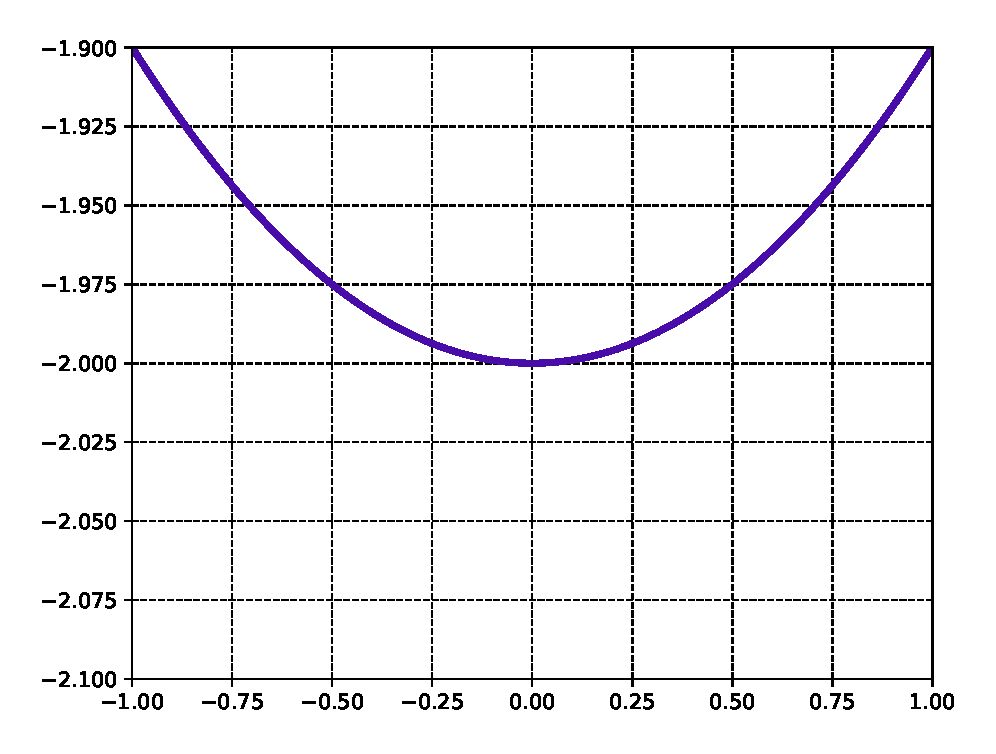
\includegraphics[width=10cm]{Graphics/limit.eps}
    \caption{}
    \label{fig:fx2}
\end{figure}
\begin{minipage}{0.45\linewidth}
    \begin{table}[H]
        \centering
        \begin{tabular}{ll}
            \hline
            \multicolumn{1}{c}{\textbf{x}} & \multicolumn{1}{c}{$\mathbf{L_i}$} \\ \hline
            -1.000000                      & -2.867921                          \\
            -0.500000                      & -10.224702                         \\
            -0.250000                      & -23.084458                         \\
            -0.125000                      & -47.538686                         \\
            -0.062500                      & -95.768898                         \\
            -0.031250                      & -191.884394                        \\
            -0.015625                      & -383.942190                        \\
            -0.007812                      & -767.971094                        \\
            -0.003906                      & -1535.985547                       \\
            -0.001953                      & -3071.992773                       \\
            -0.000977                      & -6143.996387                       \\
            -0.000488                      & -12287.998196                      \\
            -0.000244                      & -24575.999115                      \\
            -0.000122                      & -49152.000244                      \\
            -0.000061                      & -98304.005615                      \\ \hline
        \end{tabular}
        \caption{Valores obtenidos para el límite por la izquierda para una x dada.}
        \label{table:limiteizquierda}
    \end{table}
\end{minipage}
\hspace{0.5cm}
\begin{minipage}{0.45\linewidth}
    \begin{table}[H]
        \centering
        \begin{tabular}{ll}
            \hline
            \multicolumn{1}{c}{\textbf{x}} & \multicolumn{1}{c}{$\mathbf{L_s}$} \\ \hline
            1.000000                       & 2.867921                           \\
            0.500000                       & 10.224702                          \\
            0.250000                       & 23.084458                          \\
            0.125000                       & 47.538686                          \\
            0.062500                       & 95.768898                          \\
            0.031250                       & 191.884394                         \\
            0.015625                       & 383.942190                         \\
            0.007812                       & 767.971094                         \\
            0.003906                       & 1535.985547                        \\
            0.001953                       & 3071.992773                        \\
            0.000977                       & 6143.996387                        \\
            0.000488                       & 12287.998196                       \\
            0.000244                       & 24575.999115                       \\
            0.000122                       & 49152.000244                       \\
            0.000061                       & 98304.005615                       \\ \hline
        \end{tabular}
        \caption{Valores obtenidos para el límite por la derecha para una x dada.}
        \label{table:limitederecha}
    \end{table}
\end{minipage}

Observando los resultados de las tablas \ref{table:limiteizquierda} y \ref{table:limitederecha} podemos decir que el límite buscado no existe. El programa llega a la misma conclusión. En la figura \ref{fig:fx2} se puede verificar la misma conclusión.